%%%%%%%%%%%%%%%%%%%%%%%%%%%%%%%%%%%%%%%%%
%
% Optics and Radar -based observations
% Assignment 4
%
%%%%%%%%%%%%%%%%%%%%%%%%%%%%%%%%%%%%%%%%%

%----------------------------------------------------------------------------------------
%	DOCUMENT CONFIGURATIONS
%----------------------------------------------------------------------------------------

\documentclass{article}

\title{\textbf {Optics and Radar Based Observations} \\ Assignment 4\\ MIT IAP Laptop Radar Lab Exercises} % Title
\def\authorivan{Ivan \v Sinkarenko}
\def\authoranu{Anuraj Rajendraprakash}
\author{\authorivan\\\authoranu}

\usepackage{graphicx}
\usepackage{fullpage}
\usepackage{url}

% load package with ``framed'' and ``numbered'' option.
\usepackage[framed,numbered,autolinebreaks,useliterate]{mcode}

\begin{document}

\maketitle % Insert the title, author and date

\centerline{Referee: Dr. Philip J. Erickson}

\setlength\parindent{0pt} % Removes all indentation from paragraphs

\renewcommand{\labelenumi}{\alph{enumi}.} % Make numbering in the enumerate environment by letter rather than number (e.g. section 6)
\clearpage

\tableofcontents

\listoffigures

\clearpage

%----------------------------------------------------------------------------------------
%	SECTION 1. Doppler Radar Processing
%----------------------------------------------------------------------------------------

\section{Doppler Radar Processing}

\subsection{Question 1}
The Doppler shift for each target is measured from the peak location of the discrete-time Fourier transform (DTFT) of the corresponding sampled waveform. Range rate is then determined by the following formula:
\begin{equation}
\label{eq:first}
\frac{f_d}{f_c}*\frac{c}{2}
\end{equation}
where $f_d$ is the Doppler shift in Hz and $f_c$ is the center frequency of the radar in Hz. Range rate calculations will obviously be limited since shifts of the peak that are greater than $\pi$ will wrap around, resulting in incorrect calculations. Adjusting the center frequency allows the range of velocities that can be correctly calculated to change. As $f_c$ is decreased, larger speeds can be calculated, but accuracy of these velocities suffers somewhat. Conversely, as $f_c$ increased, accuracy increased, but high velocities could not be detected due to aliasing. \cite{DavenportWaters:2010dsp} Figure \ref{fig:f_c_normal} shows resulting plot with initial center frequency of 2,59 GHz, Figure \ref{fig:f_c_reduced} shows the same plot with reduced center frequency of 259 MHz, whereas Figure \ref{fig:f_c_increased} has resulting plot with increased $f_c$ of 25.9 GHz.


\begin{figure}[ht]
\begin{minipage}[b]{0.33\linewidth}
\centering
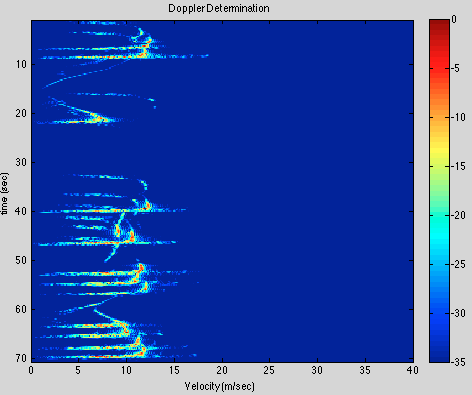
\includegraphics[width=\textwidth]{Figures/f_c_normal.png}
\caption{Doppler determination with 2.59 GHz center frequency.}
\label{fig:f_c_normal}
\end{minipage}
\begin{minipage}[b]{0.33\linewidth}
\centering
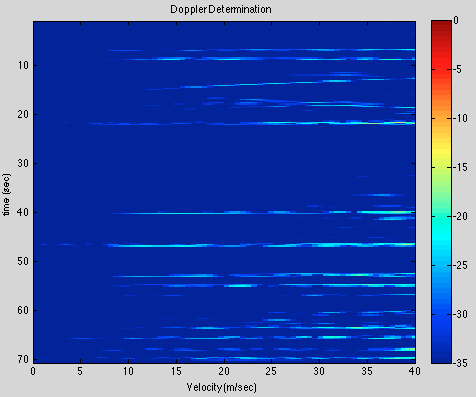
\includegraphics[width=\textwidth]{Figures/f_c_reduced.png}
\caption{Doppler determination with 259 MHz center frequency.}
\label{fig:f_c_reduced}
\end{minipage}
\begin{minipage}[b]{0.33\linewidth}
\centering
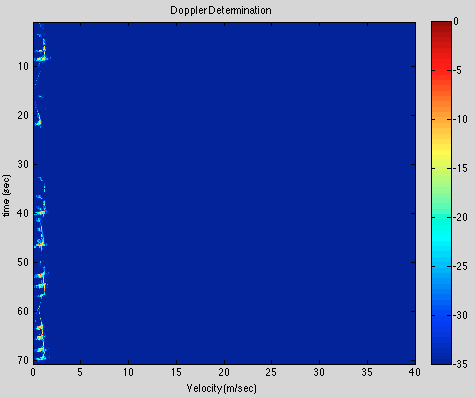
\includegraphics[width=\textwidth]{Figures/f_c_increased.png}
\caption{Doppler determination with 25.9 GHz center frequency.}
\label{fig:f_c_increased}
\end{minipage}
\end{figure}

\subsection{Question 2}

\begin{figure}[ht]
\begin{minipage}[b]{0.33\linewidth}
\centering
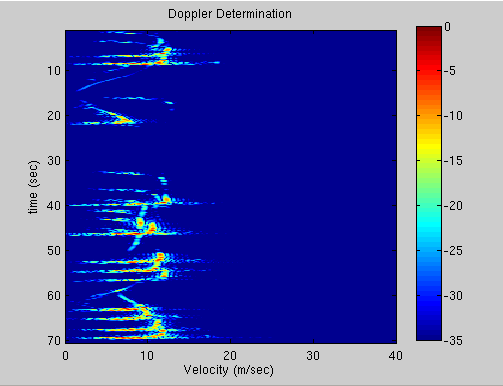
\includegraphics[width=\textwidth]{Figures/Tp_normal.png}
\caption{Doppler determination with $Tp = 0.250 $ seconds.}
\label{fig:Tp_normal}
\end{minipage}
\begin{minipage}[b]{0.33\linewidth}
\centering
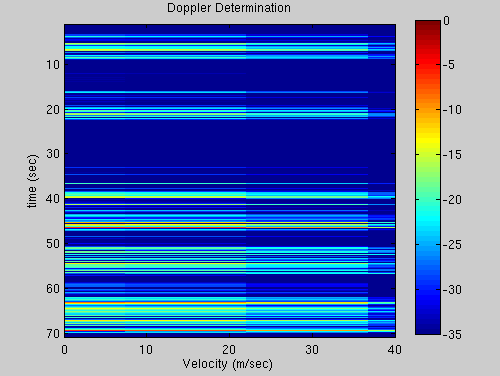
\includegraphics[width=\textwidth]{Figures/Tp_reduced.png}
\caption{Doppler determination with $Tp = 0.00250 $ seconds.}
\label{fig:Tp_reduced}
\end{minipage}
\begin{minipage}[b]{0.33\linewidth}
\centering
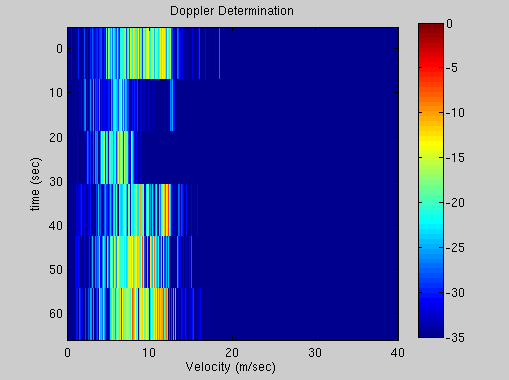
\includegraphics[width=\textwidth]{Figures/Tp_increased.png}
\caption{Doppler determination with $Tp = 10$ seconds.}
\label{fig:Tp_increased}
\end{minipage}
\end{figure}

The Figure \ref{fig:Tp_normal}, Figure \ref{fig:Tp_reduced} and Figure \ref{fig:Tp_increased} show the doppler vs time plots for Tp equal to 0.0025, 0.25 and 10 seconds respectively. It is clearly seen from the Figure \ref{fig:Tp_reduced} that as Tp is reduced the time resolustion and hence the range resolution becomes better but at the cost of doppler resolution. Also from Figure \ref{fig:Tp_increased} it is seen that an increase in Tp gives better doppler resolution but reduces the time i.e. the range resolution of the radar

\subsection{Question 3}

$zpad$ is zero padding, which should be bigger than the number of samples $N$. The Fast Fourier Transform (FFT) function adds zeros when this amount is bigger. The purpose of having zero padding is that having larger number of samples decreases $\Delta t$ of sampling, consequently increasing frequency resolution and allowing to study higher frequencies with the affordable frequency resolution without a threat to run into a aliasing. Figure \ref{fig:zpad_normal} shows Doppler determination plot with initial $zpad$ value of 8*N/2. Figure \ref{fig:zpad_reduced} represents the plot with zero padding reduced to the length of N. It is clearly seen that image resolution is worse on this plot. Figure \ref{fig:zpad_increased} contains Doppler determination plot with $zpad = 80*N/2$. It is seen that the actual resolution is similar to that in Figure \ref{fig:zpad_normal}. This means that zero padding has a upper limit after which bigger amount of zeros does not help anymore.

\begin{figure}[h!t]
\centering
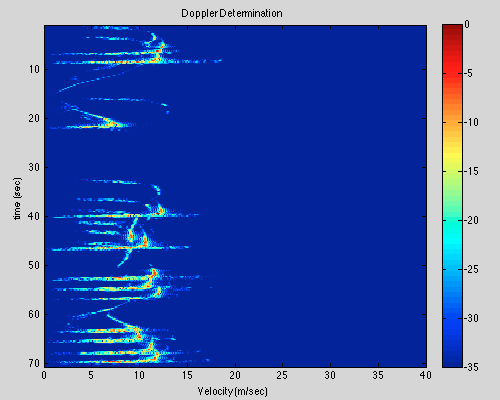
\includegraphics[width=0.7\textwidth]{Figures/zpad_normal.png}
\caption{Doppler determination with $zpad = 8*N/2$.}
\label{fig:zpad_normal}
\end{figure}
\begin{figure}[h!t]
\centering
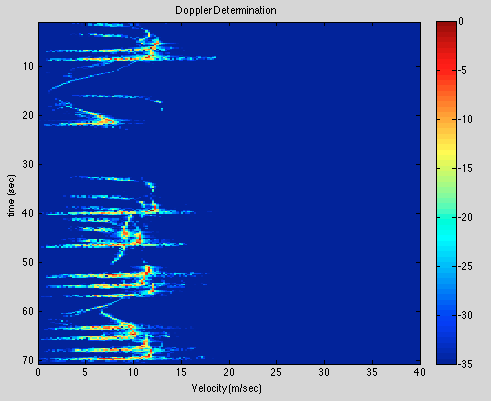
\includegraphics[width=0.7\textwidth]{Figures/zpad_reduced.png}
\caption{Doppler determination with $zpad = 2*N/2$.}
\label{fig:zpad_reduced}
\end{figure}
\begin{figure}[h!t]
\centering
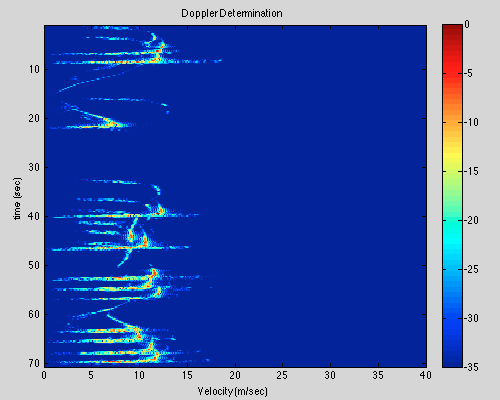
\includegraphics[width=0.7\textwidth]{Figures/zpad_increased.png}
\caption{Doppler determination with $zpad = 80*N/2$.}
\label{fig:zpad_increased}
\end{figure}


%----------------------------------------------------------------------------------------
%	SECTION 2. Range Radar Processing
%----------------------------------------------------------------------------------------

\section{Range Radar Processing}

%----------------------------------------------------------------------------------------
%	SECTION 3. CONCLUSION
%----------------------------------------------------------------------------------------
%\newpage
\section{Conclusion}

%----------------------------------------------------------------------------------------
%	SECTION 4. REFERENCES
%----------------------------------------------------------------------------------------
\newpage
\begin{thebibliography}{9}

\bibitem{Enmark:2012a3}
Enmark A.  (2012).
\newblock {\em Assignment 3. Optimization of phased array antenna radiation pattern and array configuration}.
\newblock Lule\aa \ University of Technology, Kiruna, Sweden.

\bibitem{Skolnik:2001irs}
Skolnik M. ~I.  (2001).
\newblock {\em Introduction to Radar Systems}.
\newblock The McGraw-Hill Companies, Inc., New York, United States.

\bibitem{Rottger:2000ip}
R\"ottger J.  (2000).
\newblock {\em The Instrumental Principles of MST Radars and Incoherent Scatter Radars and The Configuration of Radar System Hardware}.
\newblock Max Planck Institut F\"ur Aeronomie, Katlenburg-Lindau, Germany.

\bibitem{DavenportWaters:2010dsp}
Mark Davenport, Drew Waters (2010).
\newblock {\em Elec 431 Digital Signal Processing}.
\newblock {\url{http://www.clear.rice.edu/elec431/projects95/radar/project.html}}.

\end{thebibliography}


%----------------------------------------------------------------------------------------
%	SECTION 5. Appendix 1
%----------------------------------------------------------------------------------------
\newpage
\section{Appendix 1. Matlab code}
%\lstinputlisting{assignment.m}

%----------------------------------------------------------------------------------------
%	SECTION 6. Confirmation
%----------------------------------------------------------------------------------------
\newpage
\section{Confirmation of Participation}

This is to confirm that the members of this team participated on the investigation of the required information to solve the assignment, generated their code to perform the calculation and discussed the results.\\
\vspace{2cm}
\newline
\line(1,0){200}\\
\authorivan\\
\vspace{2cm}
\newline
\line(1,0){200}\\
\authoranu\\


\end{document}